\section{Results}\label{sec:results}
    To validate transport-independent depletion, we ran depletion simulations on
    a PWR with a single depletion zone for three cases:
    \begin{enumerate}
        \item Transport-coupled depletion,
        \item Transport-independent depletion,
        \item Transport-independent depletion with microscopic cross sections
            updated after each depletion step.
    \end{enumerate}

    The first case serves as a reference solution we use to estimate the error
    in the solution of the new method. We used 25 inactive and 125 active
    batches, with $10^6$ particles per batch. For the second case, we used three
    different group structures to test the effect on solution accuracy: one
    group, CASMO-8, and CASMO-40. The third case is much slower than the first
    case as the cross sections need to be reloaded after each depletion step.
    The third case is a sanity check that the cross sections are being computed
    correctly correctly, as it should have a smaller error than the second case.
    Due to the cross section discretization that occurs before peforming
    depletion, we do not expect the third case results to converge to the first
    case results in limit of infinite particles, but we would expect it to
    converge in the limit of infinite particles {\it and} energy groups. The
    third case only ran for one-group transport-independent depletion. 

    Tables \ref{tab:mat-params} and
    \ref{tab:mat-comps} contain the material parameters and compositions of our
    model, and Table \ref{tab:geo-params} contains the geometric parameters.  We
    used the ENDF/B-VII.1 nuclear data library available at
    \url{openmc.org/official-data-libraries}. We used the ENDF/B-VII.1 depletion
    chain in the PWR spectrum available at \url{openmc.org/depletion-chains}.
    
    \begin{table}[<options>]
        \caption{Material Parameters}
        \label{tab:mat-params}
        \begin{tabular*}{\textwidth}{@{}LLLL@{}}
            \toprule
             Item & Fuel & Cladding & Water \\ % Table header row
            \midrule
             Density [g cm$^{-3}$] & 10.4 & 6 & 1.0\\
             Volume [cm$^{3}$] & 0.1764$\pi$ & -- & -- \\
             S($\alpha$,$\beta$) & --  & -- & \verb.c_H_in_H2O.\\
        \end{tabular*}
    \end{table}

    \begin{table}[<options>]
        \caption{Material Compositions}
        \label{tab:mat-comps}
        \subfloat[Fuel Composition] {
        \begin{tabular*}{0.333\linewidth}{@{}LL@{}}
            \toprule
            Nuclide & Composition [atom \%] \\ % Table header row
            \midrule
             $^{15}$O & 0.000758 \\
             $^{16}$O & 1.999242 \\
             $^{234}$U & 0.000385 \\
             $^{235}$U & 0.043020 \\
             $^{236}$U & 0.000197 \\ 
             $^{238}$U & 0.956398 \\
        \end{tabular*}
        }
        \subfloat[Cladding Composition] {
        \begin{tabular*}{0.333\linewidth}{@{}LL@{}}
            \toprule
            Nuclide & Composition [atom \%] \\ % Table header row
            \midrule
             $^{90}$Zr & 0.5145 \\
             $^{91}$Zr & 0.1122 \\
             $^{92}$Zr & 0.1715 \\
             $^{94}$Zr & 0.1738 \\
             $^{96}$Zr & 0.028 \\ 
        \end{tabular*}
        }
        \subfloat[Water Composition] {
        \begin{tabular*}{0.333\linewidth}{@{}LL@{}}
            \toprule
            Nuclide & Composition [atom \%] \\ % Table header row
            \midrule
             $^{1}$H & 1.999689\\
             $^{2}$H & 0.000311 \\
             $^{15}$O & 0.999621 \\
             $^{16}$O & 0.000379 \\
        \end{tabular*}
        }
    \end{table}

    \begin{table}[<options>]
        \caption{Geometric Parameters}\label{tab:geo-params}
        \begin{tabular*}{\tblwidth}{@{}LLLL@{}}
            \toprule
            Fuel Radius [cm] & Clad Radius [cm] & Water Bounding Box dimensions
            [cm  $\times$ cm]\\
            \midrule
            0.42 & 0.45 &  1.24 $\times$ 1.24\\
        \end{tabular*}
    \end{table}
    Depletion is a slow process whose effects on neutronics only start to apply
    on longer timescales (days and months). For validation purposes we ran each
    of the three cases with four different magnitudes of timestep size: 360
    seconds, 4 hours, 3 days, and 30 days. All simulations ran for 10 depletion
    steps. We used the \verb.PredictorIntegrator. time stepper, which is
    analogous to the Euler method. Predictor-corrector methods are not useful
    for transport independent depletion. The correction step will utilize the
    same reaction rates as the initial prediction due to the static fluxes and
    cross sections.  This means any predictor-corrector method will produce the
    same numerical results as a predictor method but with higher floating-point
    errors due to the increased number of operations \footnote{Preliminary
    testing with predictor-corrector methods confirmed the higher floating
    point errors, however their magnitudes are marginal.}. We used constant
    reaction rate Q values multiplied by the reaction rates to obtain the
    normalization factor $f$ (\verb.fission-q. normalization) for all cases with
    a linear power density of 174 W/cm.

    The general trend in our results is that concentration errors are smaller
    for shorter depletion time steps, and larger for longer depletion time
    steps, however some nuclides exhibit more complicated behavior. 

    % actinides error 
    \begin{figure}[h!tpb]
        \centering
        \subfloat[] {
            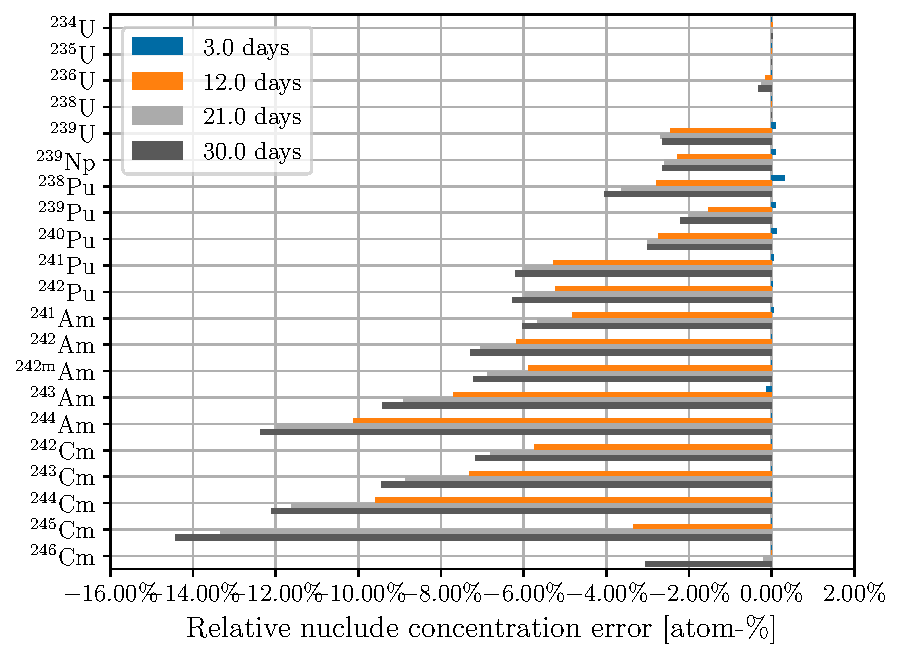
\includegraphics[width=0.5\linewidth]{figs/actinides_constant_xs_predictor_fission_q_days.pdf}
            \label{fig:actinides-error-constant-xs-days}
        }
        \subfloat[] {
            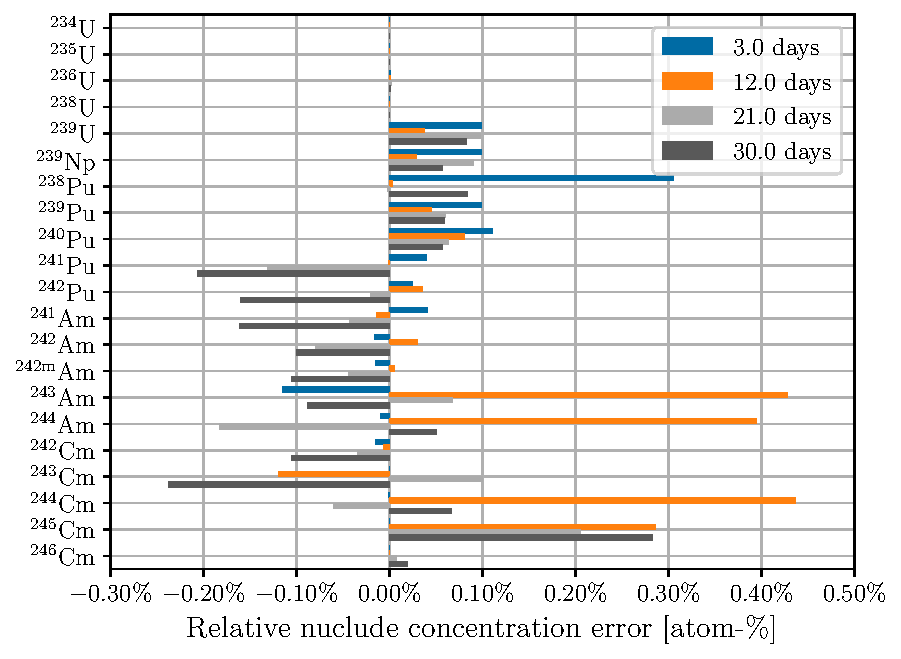
\includegraphics[width=0.5\linewidth]{figs/actinides_updating_xs_predictor_fission_q_days.pdf}
            \label{fig:actinides-error-updating-xs-days}
        }
        \caption[]{Relative actinide concentration error using 3-day time steps at 3,
                12, 21, and 30 days of depletion for
            \subref{fig:actinides-error-constant-xs-days} constant cross
            sections;
            \subref{fig:actinides-error-updating-xs-days} updating cross
            sections.}
    \end{figure}

    Figures \ref{fig:actinides-error-constant-xs-days} and
    \ref{fig:actinides-error-updating-xs-days} show the relative error in
    predicted actinide concentration for constant cross sections and updating
    cross sections, respectively, using 3-day time steps. Figures
    \ref{fig:actinides-error-constant-xs-months} and
    \ref{fig:actinides-error-updating-xs-months} show the same respective
    quantities for 30-day time steps. As expected, updating the cross sections
    at each depletion step results in low predicted nuclide concentration
    errors, on the order of a fraction of a percent. The error trend for
    constant cross sections depends both on the cross section and time step
    size. For example, constant cross sections using a 3-day time step
    underpredicts the \ce{^{241}Pu} concentration, but at longer time steps
    overpredicts the concentration. Figure \ref{fig:pu240-n-gamma-months} shows
    the overprediction is due to overcalculating the rate of ($n,\gamma$) reactions
    that occur on \ce{^{240}Pu}. 
    \begin{figure}[htpb]
        \centering
        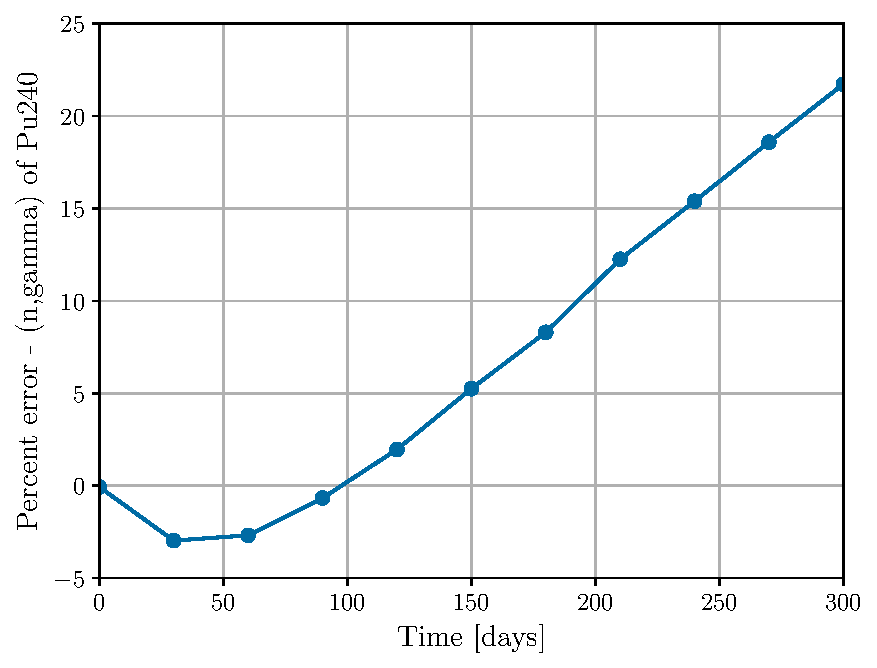
\includegraphics[width=0.5\linewidth]{figs/pu240-n-gamma-months.pdf}
        \caption{Relative \ce{^{240}Pu} ($n,\gamma$) reaction rate error using
        constant cross sections and 30-day time steps.}
        \label{fig:pu240-n-gamma-months}
    \end{figure}

    The error in \ce{^{241}Pu} concentration propogates to daughter nuclides
    that are related to the amount of \ce{^{241}Pu}, such as isotopes of \ce{Cm}
    and \ce{Am}. We observe a general trend that the less abundant
    nuclides have higher concentration error relative to transport-coupled
    depletion. The less abundant actinides have increased sensitivity to
    variations in production. The more abundant nuclides (\ce{U},
    \ce{^{239}Np}, \ce{^{239}Pu}, \ce{^{240}Pu}) tend to have low concentration
    errors, (5\% or less), whereas the less abundant actinides (isotopes of Am,
    isotopes of Cm, \ce{^{241}Pu}, \ce{^{242}Pu}) tend to have high (more
    than 10\%) concentration errors depending on the nuclide of interest.


    \begin{figure}[h!tpb]
        \centering
        \subfloat[] {
            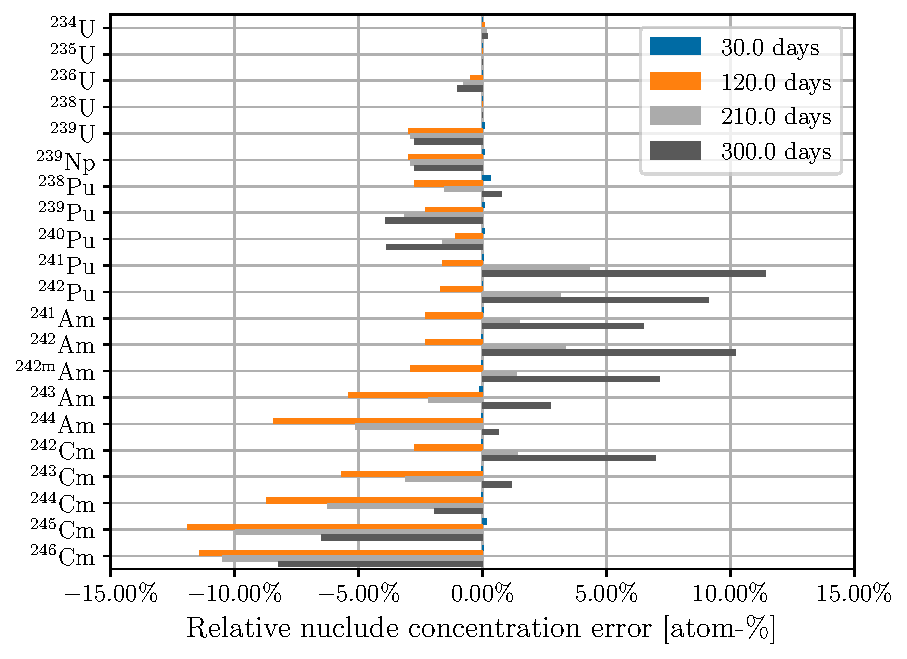
\includegraphics[width=0.5\linewidth]{figs/actinides_constant_xs_predictor_fission_q_months.pdf}
            \label{fig:actinides-error-constant-xs-months}
        }
        \subfloat[] {
            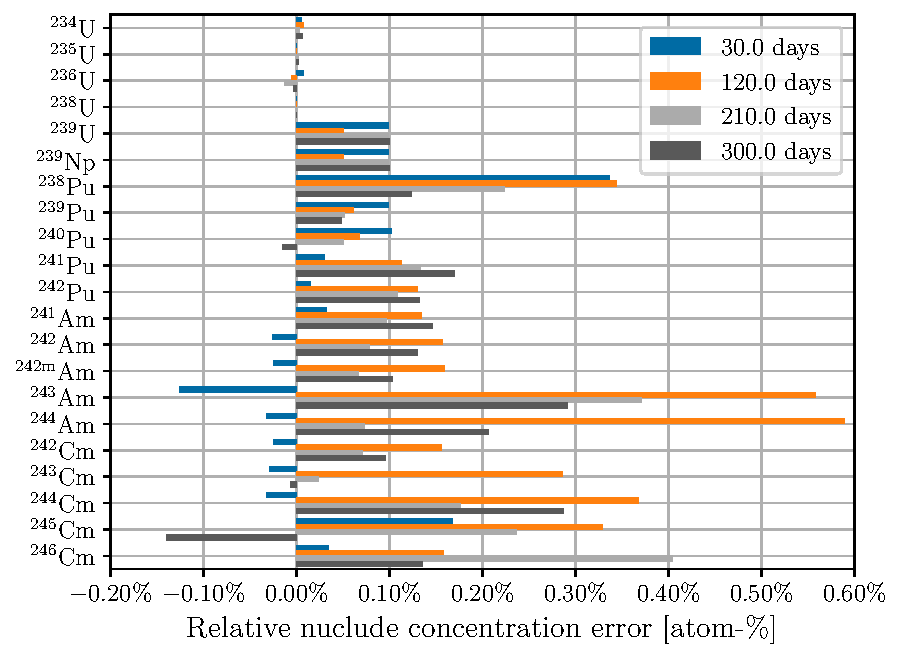
\includegraphics[width=0.5\linewidth]{figs/actinides_updating_xs_predictor_fission_q_months.pdf}
            \label{fig:actinides-error-updating-xs-months}
        }
        \caption[]{Relative actinide concentration error using 30-day time steps
            at 30,
                120, 210, and 300 months of depletion for
            \subref{fig:actinides-error-constant-xs-months} constant cross
            sections;
            \subref{fig:actinides-error-updating-xs-months} updating cross
            sections.}
    \end{figure}

    Figures \ref{fig:fp-error-constant-xs-days} and
    \ref{fig:fp-error-updating-xs-days} show the relative error in predicted
    fission product concentration using constant cross sections and updating
    cross sections, respectively, using 3-day time steps. Figures
    \ref{fig:fp-error-constant-xs-months} and
    \ref{fig:fp-error-updating-xs-months} show the same respective quantities
    for 30-day time steps. Similar to the actinides, updating the cross sections
    at each depletion step results in low predicted nuclide concentration
    errors. There is a lower concentration error across the board for
    many of these fission products compared to the actinides. This is due to the
    low concentration error of \ce{^{235}U}, which propagates to the
    fission products. Other actinides with higher concentration errors are
    orders of magnitude less abundant in the fuel than \ce{^{235}U}, so their
    effect on fission product concentration error is proportionally small.

    Concentration errors for low-abundance nuclides using 30-day time steps follow
    an interesting trend where there is an initial large negative concentration
    error that becomes more positive over time. This behavior is due to
    the static cross sections and fluxes producing the same amount of these
    nuclides every timestep, whereas in the transport-coupled case,
    net production of the low-abundance nuclides decreases over time.

    \begin{figure}[h!tpb]
        \centering
        \subfloat[] {
            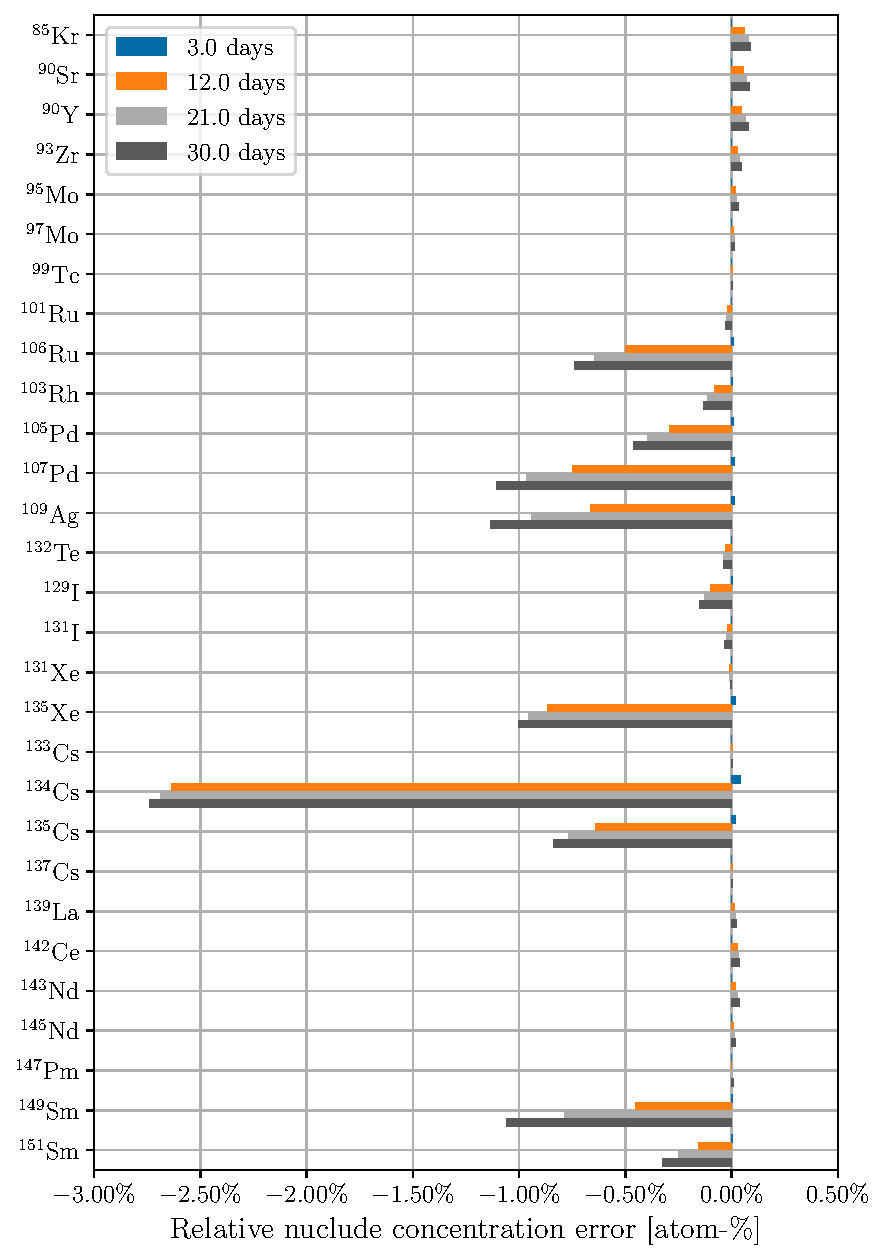
\includegraphics[width=0.5\linewidth]{figs/fission_products_constant_xs_predictor_fission_q_days.pdf}
            \label{fig:fp-error-constant-xs-days}
        }
        \subfloat[] {
            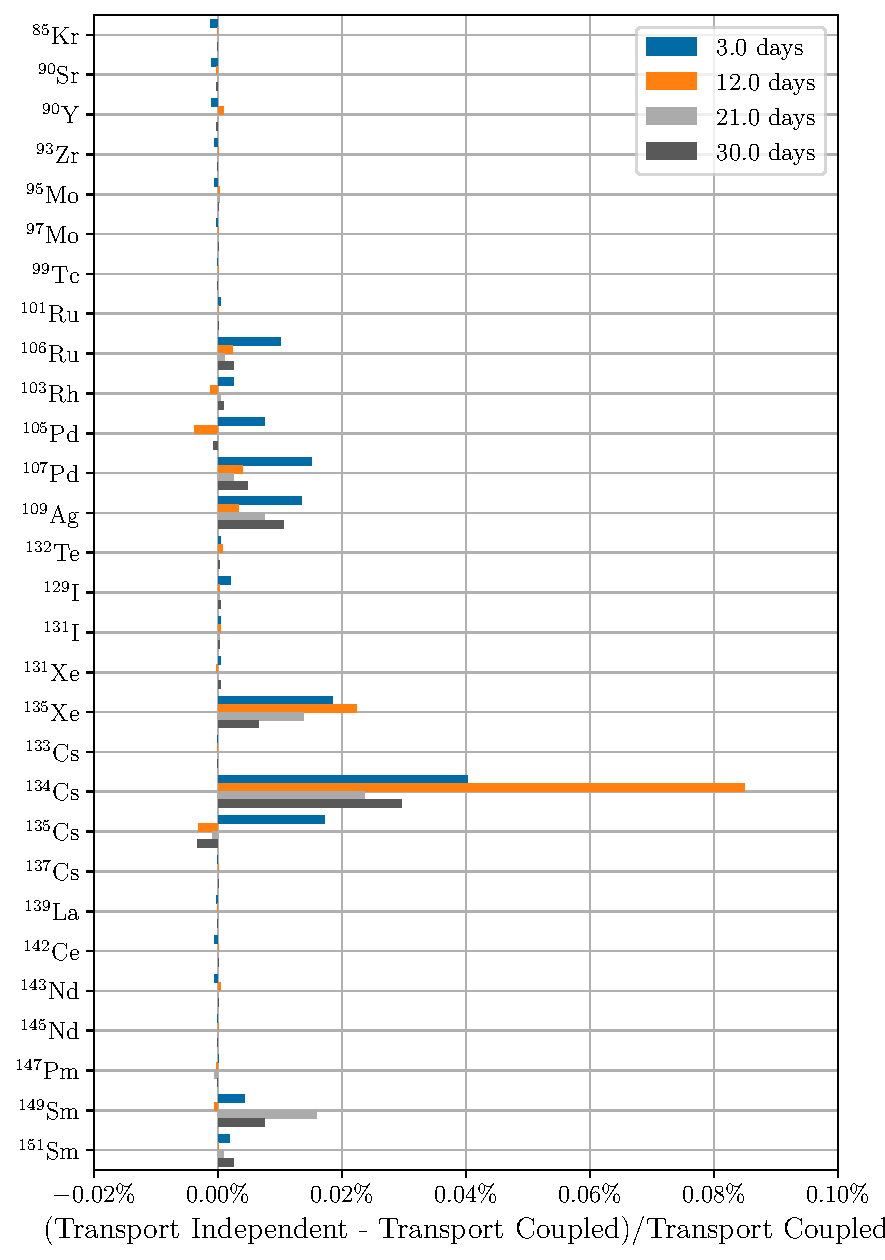
\includegraphics[width=0.5\linewidth]{figs/fission_products_updating_xs_predictor_fission_q_days.pdf}
            \label{fig:fp-error-updating-xs-days}
        }
        \caption[]{Relative fission product concentration error using 3-day time
            steps at 3, 12, 21, and 30 days of depletion for
            \subref{fig:fp-error-constant-xs-days} constant cross sections;
            \subref{fig:fp-error-updating-xs-days} updating cross sections.}
    \end{figure}

    \begin{figure}[h!tpb]
        \centering
        \subfloat[] {
            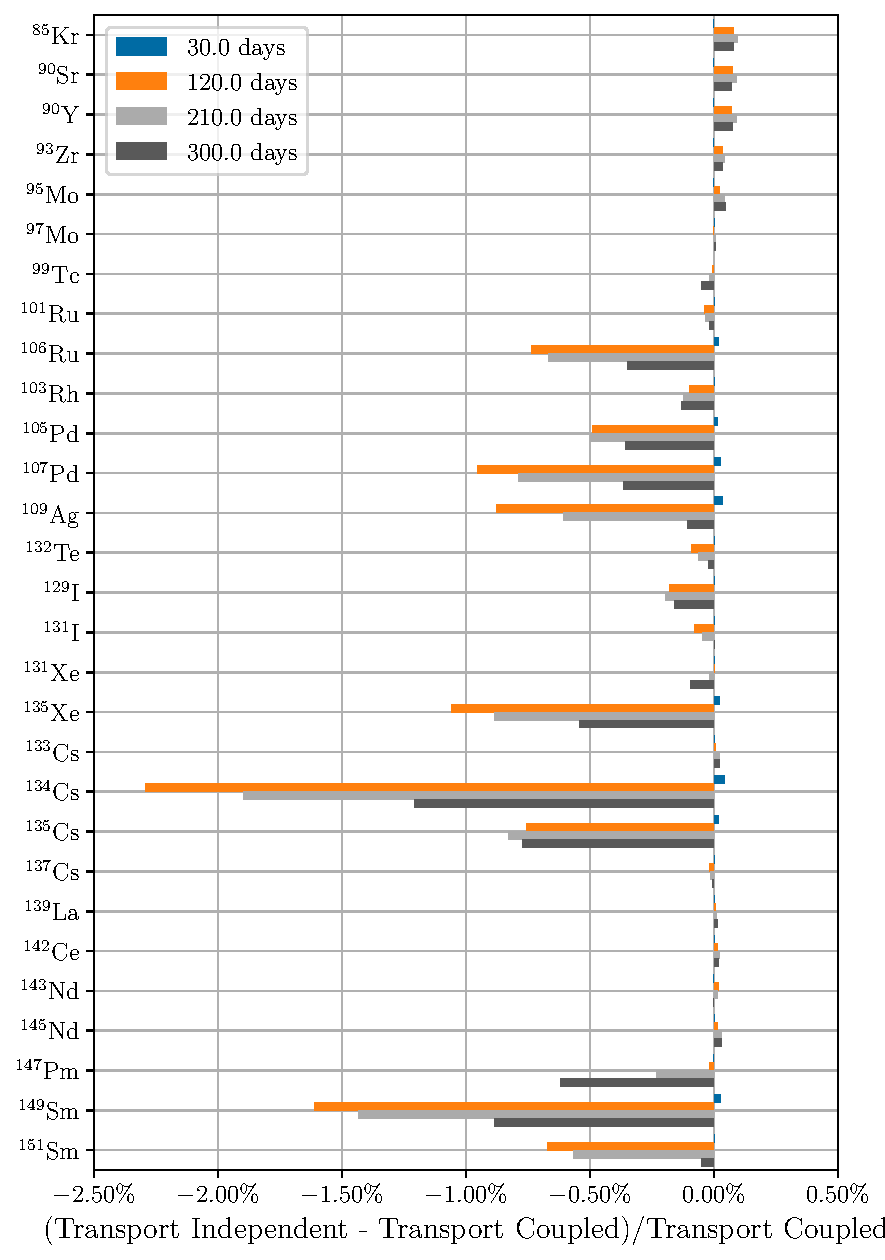
\includegraphics[width=0.5\linewidth]{figs/fission_products_constant_xs_predictor_fission_q_months.pdf}
            \label{fig:fp-error-constant-xs-months}
        }
        \subfloat[] {
            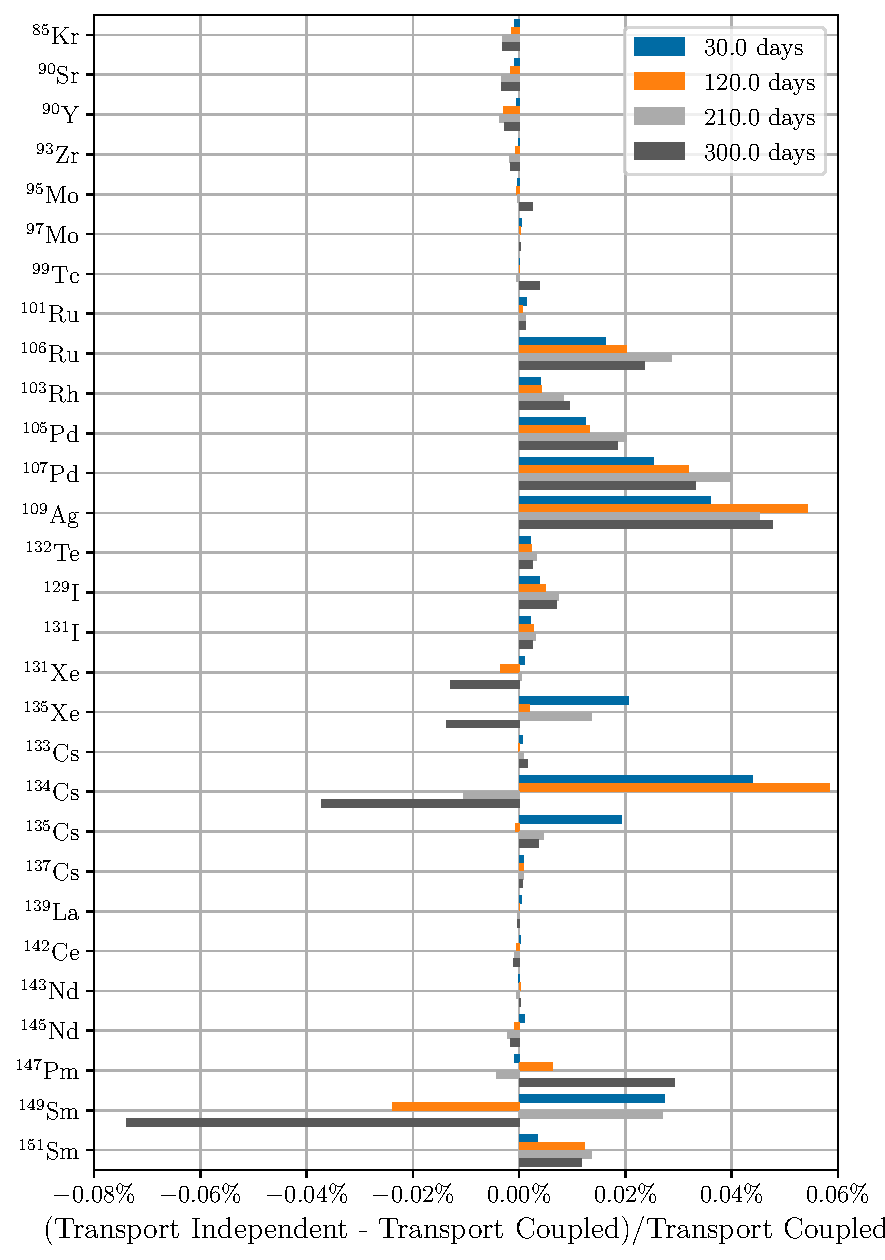
\includegraphics[width=0.5\linewidth]{figs/fission_products_updating_xs_predictor_fission_q_months.pdf}
            \label{fig:fp-error-updating-xs-months}
        }
        \caption[]{Relative fission product concentration error using 30-day
            time steps at 30, 120, 210, and 300 months of depletion for
            \subref{fig:fp-error-constant-xs-months} constant cross sections;
            \subref{fig:fp-error-updating-xs-months} updating cross sections.}
    \end{figure}

    Repeating this analysis for both the CASMO-8 and CASMO-40 multi-group
    structures did not yield noticeable decreases in nuclide concentration
    errors for transport-independent depletion over the one-group case.  Figures
    \ref{fig:actinides-error-casmo8-xs-days} and
    \ref{fig:actinides-error-casmo40-xs-days} show the relative error in
    predicted actinide concentration using the CASMO-8 and CASMO-40 group
    structures, respectively, using 3-day time steps. Figures
    \ref{fig:actinides-error-casmo8-xs-months} and
    \ref{fig:actinides-error-casmo40-xs-months} show the same respective
    quantities for 30-day time steps.  It is possible in more complex models,
    like full reactor depletion, that the multi-group structure could become more
    important.

    \begin{figure}[htpb]
        \centering
        \subfloat[] {
            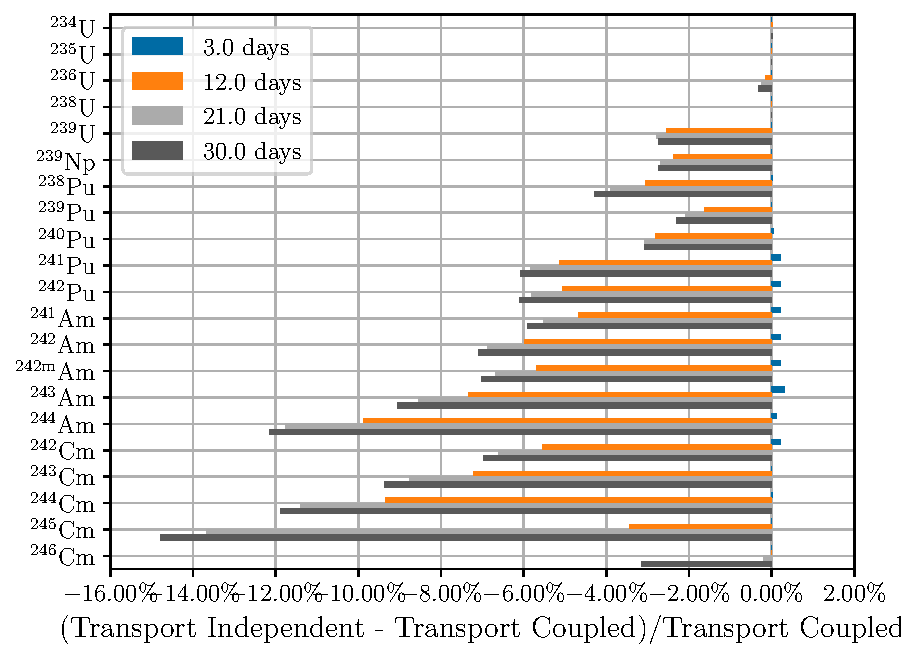
\includegraphics[width=0.5\linewidth]{figs/actinides_casmo8_constant_xs_predictor_fission_q_days.pdf}
            \label{fig:actinides-error-casmo8-xs-days}
        }
        \subfloat[] {
            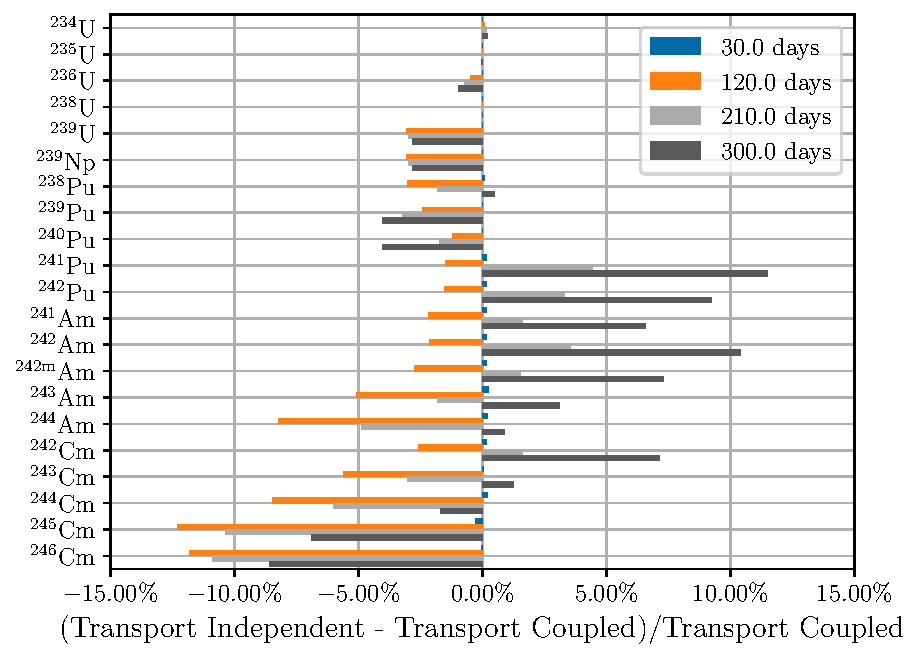
\includegraphics[width=0.5\linewidth]{figs/actinides_casmo8_constant_xs_predictor_fission_q_months.pdf}
            \label{fig:actinides-error-casmo8-xs-months}
        }\\
        \subfloat[] {
            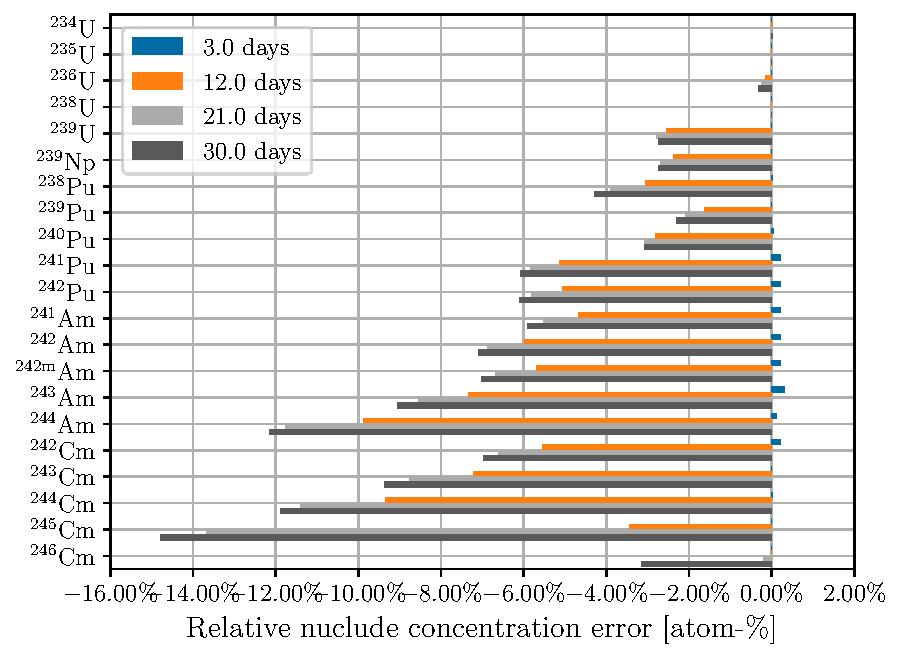
\includegraphics[width=0.5\linewidth]{figs/actinides_casmo40_constant_xs_predictor_fission_q_days.pdf}
            \label{fig:actinides-error-casmo40-xs-days}
        }
        \subfloat[] {
            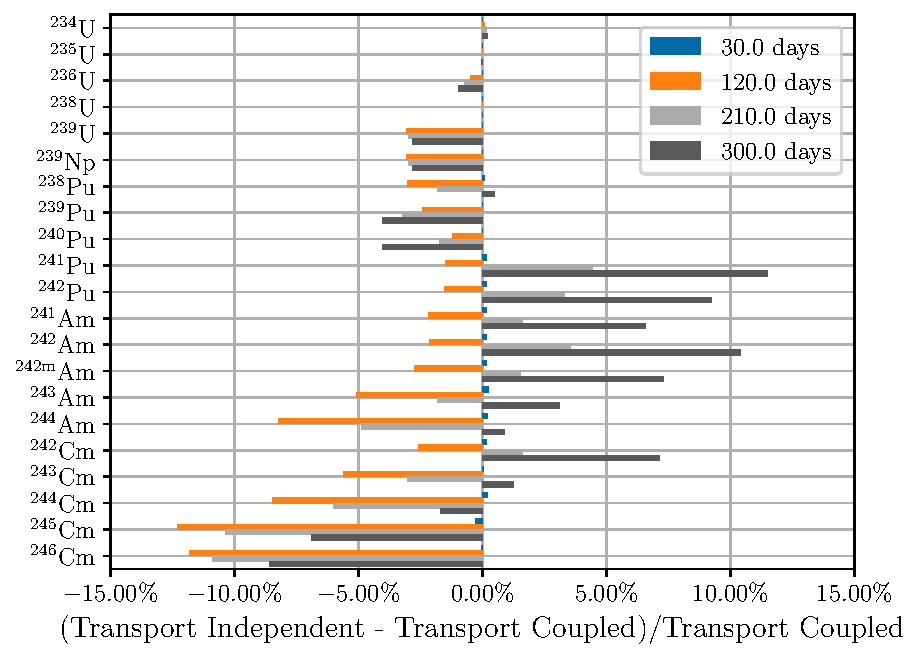
\includegraphics[width=0.5\linewidth]{figs/actinides_casmo40_constant_xs_predictor_fission_q_months.pdf}
            \label{fig:actinides-error-casmo40-xs-months}
        }
        \caption[]{Relative actinide concentration error using constant cross
                sections and 3-day time steps at 3, 12, 21, and 30 days of
                depletion for the
            \subref{fig:actinides-error-casmo8-xs-days} CASMO-8 group
                structure;
            \subref{fig:actinides-error-casmo40-xs-days} CASMO-40 group
                structure;
            and 30-day time steps at 30, 120, 210, and 300 days of
                depletion for the
            \subref{fig:actinides-error-casmo8-xs-months} CASMO-8 group
                structure;
            \subref{fig:actinides-error-casmo40-xs-months} CASMO-40
            group structure.}
    \end{figure}

    The transport-coupled simulations each took several hours to complete,
    whereas the transport-independent simulations using
    \verb.IndependentOperator. took seconds to minutes to complete.
